\scanpage{90}
\mspage{- 19 -}
\uline{Preuve} : Soit $R$ le crible engendré par les $(U_i\mathrel{\text{---}\!\handwritten{>}}X)$. Le faisceau associé à $R$ est isomorphe au faisceau associé à $X$. On applique alors la proposition précédente et la formule (19).
% A pencil paragraph-break sign precedes « Cette ».
\handwritten{\raisebox{.3ex}{\begin{tikzpicture}[x=.6em,y=.4em]\draw (0,0)--(.7,0)--(.7,1)--(1.6,1);\end{tikzpicture}}}
Cette suite spectrale est \deleted{dûe à} \inserted{\handwritten{celle de}} Cartan-Leray.

\margin{\handwritten{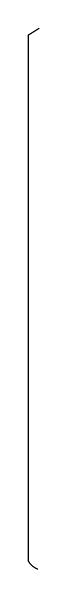
\begin{tikzpicture}[x=1em,y=1em]\draw (.4,.25)--(0,0)--(0,-19) to[bend right=18] (.35,-19.3);\end{tikzpicture}}}
\uline{Corollaire 2.5} : Il existe une suite spectrale fonctorielle en $F$ et en $X$ (objet de $C$) :
\[
 H^{p+q}(C^{\handwritten{\sim}}/X,F)\handwritten{\Longleftarrow}
 \overset{\handwritten{\scriptscriptstyle\vee}}{H}{}^p(X,\handwritten{\mathscr H}^q(F))
\]
Cette suite spectrale fournit, lorsque $X$ varie dans $C$, la suite spectrale de préfaisceaux :
\[
 \handwritten{\mathscr H}^{p+q}(F)\handwritten{\Longleftarrow}
 \handwritten{\check{\mathscr H}}^p(\handwritten{\mathscr H}^q(F))
\]
Ces suites spectrales fournissent des morphismes fonctoriels \handwritten{:}
\margin{\handwritten{$\unsure{\checkmark}$}}
\[
\begin{aligned}
\handwritten{\Phi}^q(F)&:\handwritten{\check{\mathscr H}}^q(\handwritten{\mathscr H}^0(F))\handwritten{\longrightarrow}\handwritten{\mathscr H}^q(F)\\
\handwritten{\Phi}^q_X(F)&:\overset{\handwritten{\scriptscriptstyle\vee}}{H}{}^q(\unsure{E|S}\ X,\handwritten{\mathscr H}^0(F))\handwritten{\longrightarrow}H^q(X,F)
\end{aligned}
\]
Les morphismes $\handwritten{\Phi}^q$ et $\handwritten{\Phi}^q_X$ sont des isomorphismes lorsque $q$ égale $0$ ou $\handwritten{1}$. Les morphismes $\handwritten{\Phi}^2$ et $\handwritten{\Phi}^2_X$ sont des monomorphismes. Plus généralement, lorsque les préfaisceaux $\handwritten{\mathscr H}^i(F)$ sont nuls pour $0\handwritten{<}i\handwritten{<}n$, les morphismes $\handwritten{\Phi}^q(F)$ et $\handwritten{\Phi}^q_X(F)$ sont des isomorphismes pour $0\handwritten{\leq}q\handwritten{\leq}n$ et des monomorphismes pour $q=n+1$.

\uline{Preuve} : La première suite spectrale s'obtient en passant à la limite inductive dans la suite spectrale de la proposition 2.3 sur les

\hfill .../...

% archive sheet number: 89
